%
%
%
\section{Cadmium Telluride Sensor}
\label{sec:siliconpad}
%Fig: Quantum Efficiency vs wavelength
%Photos of sensor, drawing for the circuit
The semi-conducting properties of Cadmium-Telluride has been studied since many decades \cite{cdtegeneric}, 
in particular in the the context of using the material in photo voltaic applications.
Cadmium-telluride sensor are widely used in xray detectors \cite{cdtesensorsgeneric,cdtesensors1,cdtesensors2,cdtesensors3}. 
They have also been investigated for synchrotron radaition detectors in accelerator technology \cite{cdtelhc}.   
In our previous 
studies~\cite{Anderson:2015gha,MCPShowerMaxPaper,Ronzhin201552,SiliconTiming,PixelatedMCP,Anderson:2016ygg,Anderson:2015tia} 
we have demonstrated that increasing the primary sensor signal is crucial to achieve good timing resolutions.  
Cadmium-telluride features a significantly larger efficiency for detecting photons in the $10-100$~keV energy range 
compared to silicon sensors. The higher atomic number of Cadmium and Tellurium, averaging to 48.52 for the compound bulk material, results in a higher interaction cross section for photons in this energy range. 
Photons with such energies are abundant in electromagnetic showers \cite{showercomposition}. 
Furthermore, CdTe sensor are available with thicknesses of 1 mm and more. 
The path-length of the charged shower particles in the sensor material scales accordingly, 
resulting in a larger primary signal.
%
Our measurements were conducted with a CdTe Schottky type diode purchased from Acrorad \cite{acrorad}. 
It is \unit{cm}^{2} in transverse size and 1 mm thick.
It was operated at a bias voltage of 700 V and the dark current was between $3$~nA 
and $6$~nA depending on the environmental conditions in the test beam experimental 
zones.     
%
\begin{figure}[htbp] 
\centering
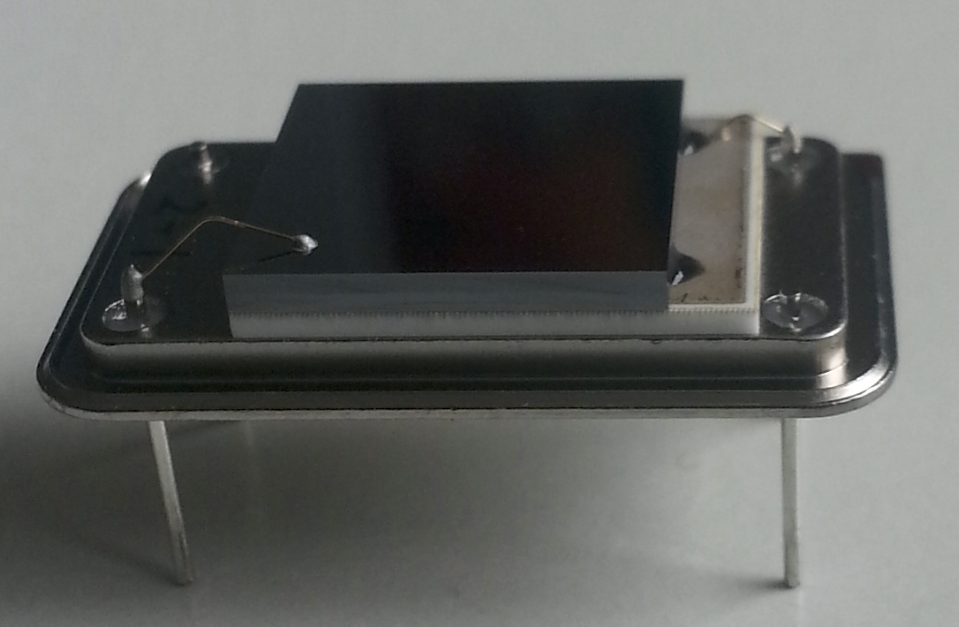
\includegraphics[width=0.49\textwidth]{figures/CdTeSensor.png} 
\caption{CdTe sensor used in the setup. The sensor is a Shottky type diode with a transverse size 
of $1$~$\unit{cm}^{2}$ and a thicknees of 1 mm. It is biased at 700 V. 
On the front, left corner of the sensor the wire bond connection 
to the metalized top layer of the sensor can be seen.} 
\label{fig:CdTeSensor} 
\end{figure} 
%
The sensor was placed in a box made of 0.3 mm copper sheets sealed with copper tape. 
The electrical circuit shown in Fig.~\ref{fig:cdtecircuit} was used to connect to the sensor to the bias 
voltage with a standard high voltage cable and the readout electronics using a SMA cable with a feed 
through penetrating the copper box.
A $36$~dB high bandwidth amplifier from Hamamatsu was used to amplify the output signal of the CdTe sensor.
A $10$~dB attenuator was used to attenuate the input signal to the amplifier to adjust the CdTe signal 
to the dynamic range of the amplifier. The output of the amplifier was connected into a 
CAEN V1742 digitizer operated at 5 GS/s.
%
\begin{figure}[htbp] 
\centering
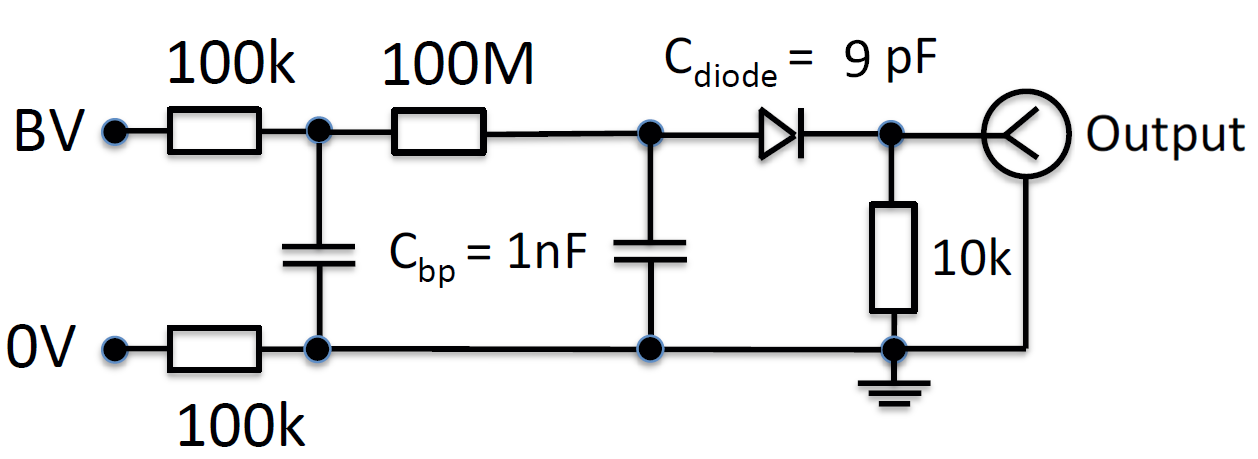
\includegraphics[width=0.49\textwidth]{figures/circuit_CdTe.png} 
\caption{Schematic of the circuit used to polarize and read out the 
CdTe sensor. The circuit and the sensor are enclosed in a copper box.} 
\label{fig:cdtecircuit} 
\end{figure} 
%
